\section{Evaluation of Model}
Having now defined all needed templates as to model a factory configuration in UPPAAL, we would like to evaluate our design. First we will evaluate, how well our model is capable of emulating reality. This is done by comparing the time it takes for a real life factory configuration to produce an order items, to the rating we give the same configuration when simulated in UPPAAL. Furthermore, we will also evaluate how efficient our implementation is, when it comes to rating a configuration. This is done, by seeing how the state space and search time for fastest traces increase, as we increase the complexity of the configuration and order. \todo{Update hvis vi ikke kigger på kompleksistet}

\subsection{The Model Compared to Reality} 
In order to compare our model to reality, we set up the configuration of the actual CP Learning Factory mentioned earlier using our UPPAAL templates. We then run different orders on both the actual factory and the model. Afterwards, we compare the time it takes for both to produce their orders.  

The configuration, which we wish to simulate, is used to produce faux smartphones. 3 different recipes were set up, which described different types of smartphones that the configuration may produce. These can be seen in \cref{fig:cp-recipes}. Each are named after, how many fuses are put into them.

\begin{figure}[h]
\centering
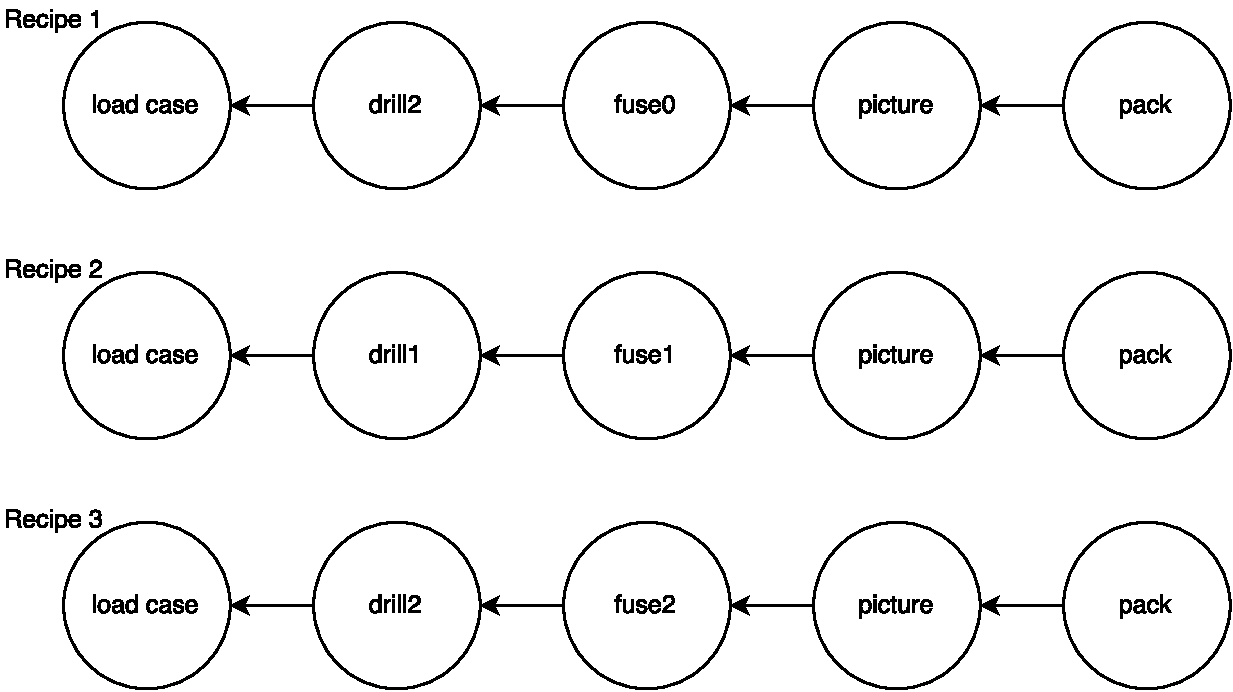
\includegraphics[width=0.5\textwidth]{cp-recipes.pdf}
\caption{Dependency graphs representing the three recipes the CP-Factory could produce}
\label{fig:cp-recipes}
\end{figure}

Inspecting the configuration, we find the different modules and the types of work that they may perform, as well as how they connect. This is shown in \cref{fig:cp-setup}. We choose to disregard that these modules each have two conveyor belts, as both are not used by any item produced. We also disregard the \textit{Transport1} module, as it is not used in the production of any item.

\begin{figure}[h]
\centering
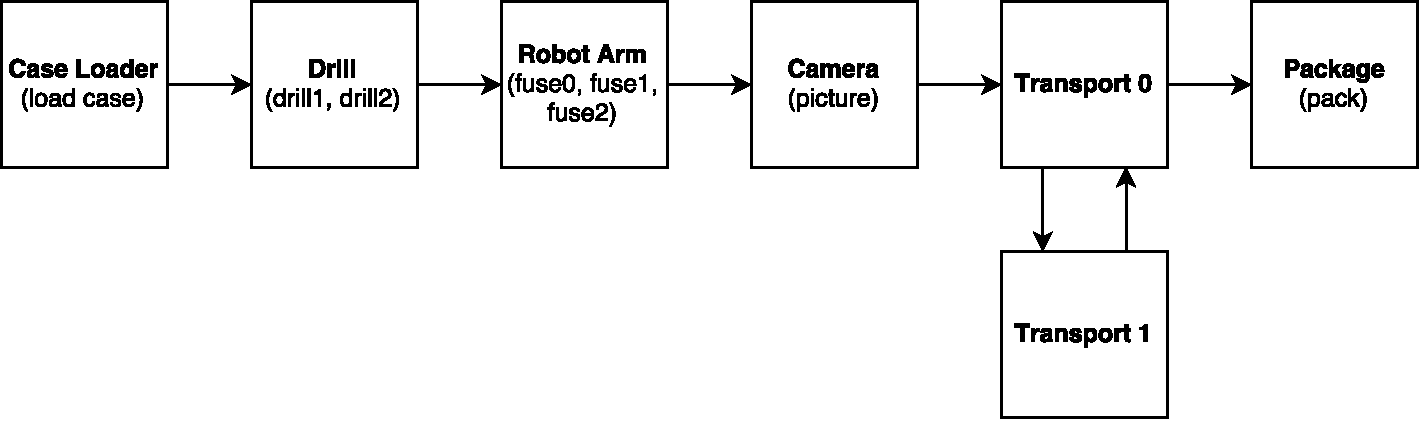
\includegraphics[width=\textwidth]{cp-setup.pdf}
\caption{Graphical representation of the CP-Factory configuration at Aalborg University}
\label{fig:cp-setup}
\end{figure}

Each item is placed on the configuration in the \textit{Case Loader} module and are removed at the \textit{Package} module. We were allowed to try and produce some items using the factory. Here we timed how long it takes for items to pass over modules, and how long it takes for certain works to be done. Averages of these times are listed in \cref{tab:cp-time}.

\begin{table}[]
\centering
\begin{tabular}{ccccc}
\multicolumn{1}{l}{} & \multicolumn{1}{l}{PLACE HOLDER} & \multicolumn{1}{l}{TABLE} & \multicolumn{1}{l}{PLACE} & \multicolumn{1}{l}{HOLDER} \\
recipe 1             & 69                               & 69                        & 69                        & 69                         \\
recipe 2             & 69                               & 69                        & 69                        & 69                         \\
recipe 3             & 69                               & 69                        & 69                        & 69                        
\end{tabular}
\caption{Table showing the time it took for transport through and do different kinds of work on modules. Times are in milliseconds}
\label{tab:cp-time}
\end{table}

In total we ran four different orders on the configuration. On \cref{tab:orders} each order is defined by the item types it needs to produce, as well as the amount of each type required.   

\begin{table}[htb]
\centering
\begin{tabular}{|l|l|}
\hline
{\ul \textbf{Order Name}} & {\ul \textbf{Description}}                                                    \\ \hline
\textbf{SingleNoFuse}     & NoFuse: 1                                                                     \\ \hline
\textbf{SingleLeftFuse}   & LeftFuse: 1                                                                   \\ \hline
\textbf{SingleBothFuse}   & BothFuse: 1                                                                   \\ \hline
\textbf{AllTypes}         & \begin{tabular}[c]{@{}l@{}}NoFuse: 1\\ LeftFuse: 1\\ BothFuse: 1\end{tabular} \\ \hline
\end{tabular}
\caption{Describes each order by the item types to produce as well as the amount of each.}
\label{tab:orders}
\end{table}


With all this in place, we are able to set up the configuration in UPPAAL using our templates and running each of the four orders on it. In \cref{app:festoex} is shown how we set up the system to run the \textit{AllTypes} order. Please note that the \textit{Item} template is here called \textit{Recipe} and similarly \textit{ItemQueue} is called \textit{RecipeQueue}. The variables \textit{recipe0}, \textit{recipe1} and \textit{recipe2} refer to the 3 processes, which represent the three items that need to be produced for the \textit{AllTypes} order. At the bottom of the example, we see how we parallelize all the smaller processes into one big system process. For this case the following reachability query is given to the UPPAAL model checker:
\\ \\
$E<>\textit{ }recip0.done\textit{ and }recipe1.done\textit{ and }recipe2.done$
\\ \\
It asks: \textit{"From the initial state, can we reach a state where all three items have been completed"}. A similar query is used for the three simpler orders. In all cases it evaluates to true. Because of this we can produce the shortest timed trace for each order, and on the last state read the value of the global clock. This is the configuration's rating given the specific order, which describes how long it takes to run the fastest schedule. Having extracted this from each of the four orders, we compare them with the time it takes to complete the orders on the actual factory configuration. The results of this can be seen in \cref{tab:cp-results}.

\begin{table}[htb]
\centering
\begin{tabular}{|l|l|l|l|}
\hline
{\ul \textbf{Order Name}} & {\ul \textbf{Actual}} & {\ul \textbf{Simulated}} & {\ul \textbf{Difference}} \\ \hline
\textbf{SingleNoFuse}     & 144.8                 & 144.9                    & 0.1                       \\ \hline
\textbf{SingleLeftFuse}   & 156.5                 & 156.6                    & 0.1                       \\ \hline
\textbf{SingleBothFuse}   & 171.6                 & 171.7                    & 0.1                       \\ \hline
\textbf{AllTypes}         & 305                   & 311                      & 6                         \\ \hline
\end{tabular}
    \caption{Comparison of actual and simulated times. Time is in milliseconds.}
    \label{tab:cp-results}
\end{table}

Looking at the results, we are almost spot on for the very simple orders. Yet the simulated and actual time drift a bit apart as the orders becomes more complex, though still to a small degree in our case. These results will be discussed further in \cref{sec:modeling}.

\subsection{The Complexity of the Model}